
\documentclass[tikz, border=10pt]{standalone}
\usepackage{tikz}
\usetikzlibrary{positioning, chains, shapes.geometric, fit, shapes, arrows.meta, calc, backgrounds}

\begin{document}
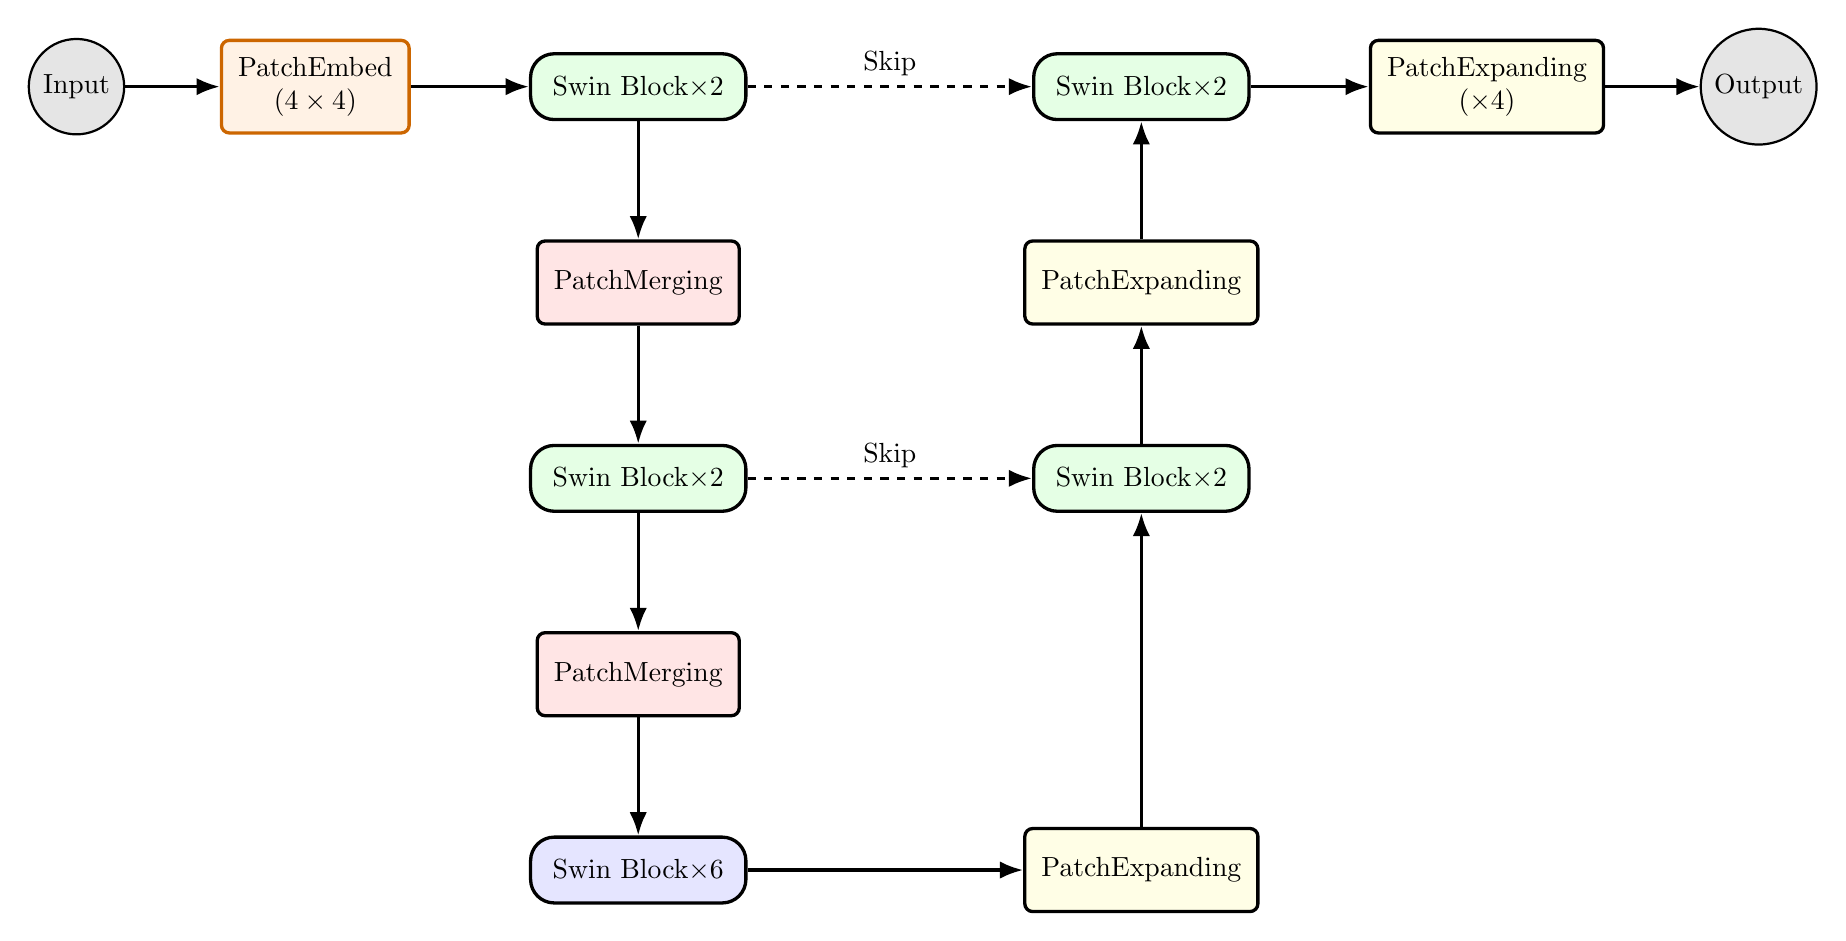
\begin{tikzpicture}[
    >=LaTeX, 
    very thick,
    node distance=1.0cm and 1.2cm,
    arrow/.style={
        ->,
        very thick,
        rounded corners=0.2cm
    },
    block/.style={
        rectangle,
        fill=gray!10,
        rounded corners=3mm,
        draw,
        very thick,
        inner sep=0.8em
    },
    layer/.style={
        rectangle,
        fill=white!10,
        rounded corners=1mm,
        inner xsep=0.6em,
        inner ysep=0.6em,
        minimum height=3.0em,
        align=center,
        draw,
        very thick
    },
    conv/.style={
        layer,
        fill=orange!10,
        draw=orange!80!black
    },
    relu/.style={
        layer,
        fill=yellow!10,
        draw=yellow!80!black,
        minimum height=2.5em
    },
    pool/.style={
        layer,
        fill=red!10,
        draw=red!80!black
    },
    input/.style={ 
        circle,
        minimum width=3.0em,
        draw,
        fill=gray!20,
        thick,
        align=center
    },
    sum/.style={
        circle,
        draw,
        fill=white,
        inner sep=0pt,
        minimum size=1.2em,
        node contents={+}
    }
]


    % Input
    \node[input] (in) {Input};

    % --- Encoder ---
    
    % Patch Embed
    \node[conv, right=of in] (pe) {PatchEmbed\\($4\times 4$)};
    \draw[arrow] (in) -- (pe);

    % Encoder Stage 1
    \node[block, right=1.5cm of pe, fill=green!10] (enc1) {Swin Block\\$\times 2$};
    \draw[arrow] (pe) -- (enc1);

    % Patch Merging 1 (Down)
    \node[layer, below=1.5cm of enc1, fill=red!10] (merge1) {PatchMerging};
    \draw[arrow] (enc1.south) -- (merge1.north);

    % Encoder Stage 2
    \node[block, below=1.5cm of merge1, fill=green!10] (enc2) {Swin Block\\$\times 2$};
    \draw[arrow] (merge1) -- (enc2);

    % Patch Merging 2
    \node[layer, below=1.5cm of enc2, fill=red!10] (merge2) {PatchMerging};
    \draw[arrow] (enc2) -- (merge2);

    % Bottleneck
    \node[block, below=1.5cm of merge2, fill=blue!10] (bot) {Swin Block\\$\times 6$};
    \draw[arrow] (merge2) -- (bot);

    % --- Decoder ---

    % Patch Expanding 2 (Up - align right)
    \node[layer, right=3.5cm of bot, fill=yellow!10] (expand2) {PatchExpanding};
    \draw[arrow] (bot) -- (expand2);

    % Decoder Stage 2
    \node[block, at={(expand2 |- enc2)}, fill=green!10] (dec2) {Swin Block\\$\times 2$};
    \draw[arrow] (expand2) -- (dec2);

    % Skip 2
    \draw[arrow, dashed] (enc2.east) -- node[above]{Skip} (dec2.west);

    % Patch Expanding 1
    \node[layer, at={(dec2 |- merge1)}, fill=yellow!10] (expand1) {PatchExpanding};
    \draw[arrow] (dec2) -- (expand1);

    % Decoder Stage 1
    \node[block, at={(expand1 |- enc1)}, fill=green!10] (dec1) {Swin Block\\$\times 2$};
    \draw[arrow] (expand1) -- (dec1);

    % Skip 1
    \draw[arrow, dashed] (enc1.east) -- node[above]{Skip} (dec1.west);

    % Output
    \node[layer, right=1.5cm of dec1, fill=yellow!10] (final_expand) {PatchExpanding\\($\times 4$)};
    \node[input, right=of final_expand] (out) {Output};
    
    \draw[arrow] (dec1) -- (final_expand);
    \draw[arrow] (final_expand) -- (out);

\end{tikzpicture}
\end{document}
